% ============================================================
% SEMINAR HASIL TESIS
% Restorasi Dokumen Terdegradasi Menggunakan GAN
% dengan Diskriminator Dual-Modal dan Optimasi Loss Function
% Berorientasi HTR
% ============================================================
% Ukuran slide standar: 16:9 (widescreen) - 160mm x 90mm
% Alternatif: aspectratio=43 untuk 4:3 tradisional (128mm x 96mm)
\documentclass[aspectratio=169,10pt,t]{beamer}

% Geometry untuk slide 16:9 (sudah default di beamer)
% Ukuran efektif: 160mm x 90mm (atau 16cm x 9cm)

% ============================================================
% THEME AND COLORS
% ============================================================
\usetheme{Madrid}
\usecolortheme{seahorse}

% Pengaturan ukuran font lebih kecil untuk menghindari overflow
\setbeamerfont{frametitle}{size=\normalsize}
\setbeamerfont{block title}{size=\small}
\setbeamerfont{block body}{size=\small}

% Custom colors
\definecolor{itbblue}{RGB}{0,61,121}
\definecolor{itbgold}{RGB}{180,151,90}
\definecolor{darkgreen}{RGB}{0,100,0}
\definecolor{darkred}{RGB}{139,0,0}
\definecolor{lightgray}{RGB}{240,240,240}

\setbeamercolor{palette primary}{bg=itbblue,fg=white}
\setbeamercolor{palette secondary}{bg=itbblue!80,fg=white}
\setbeamercolor{palette tertiary}{bg=itbblue!60,fg=white}
\setbeamercolor{structure}{fg=itbblue}
\setbeamercolor{title}{fg=itbblue}
\setbeamercolor{frametitle}{bg=itbblue!10,fg=itbblue}
\setbeamercolor{block title}{bg=itbblue,fg=white}
\setbeamercolor{block body}{bg=lightgray}
\setbeamercolor{block title alerted}{bg=darkred,fg=white}
\setbeamercolor{block title example}{bg=darkgreen,fg=white}

% ============================================================
% PACKAGES
% ============================================================
\usepackage[utf8]{inputenc}
\usepackage[T1]{fontenc}
\usepackage[bahasa]{babel}
\usepackage{graphicx}
\usepackage{amsmath,amssymb}
\usepackage{booktabs}
\usepackage{multirow}
\usepackage{array}
\usepackage{tikz}
\usepackage{xcolor}
\usepackage{fontawesome5}
\usepackage{subcaption}
\usepackage{adjustbox}

\usetikzlibrary{shapes,arrows,positioning,calc,decorations.pathreplacing}

% ============================================================
% SETTINGS
% ============================================================
\setbeamertemplate{navigation symbols}{}
\setbeamertemplate{footline}[frame number]
\setbeamersize{text margin left=6mm,text margin right=6mm}

% Pengaturan untuk menghindari overflow pada slide
\setlength{\parskip}{0.3em}
\renewcommand{\baselinestretch}{0.95}

% ============================================================
% TITLE PAGE INFO
% ============================================================
\title[Restorasi Dokumen GAN-HTR]{%
    \textbf{Restorasi Dokumen Terdegradasi Menggunakan}\\
    \textbf{Generative Adversarial Network dengan}\\
    \textbf{Diskriminator Dual-Modal dan Optimasi}\\
    \textbf{Loss Function Berorientasi HTR}}

\author[Jatniko N. M.]{%
    \textbf{Jatniko Nur Mutaqin}\\
    \small NIM: 23523314}

\institute[ITB]{%
    Program Studi Magister Informatika\\
    Institut Teknologi Bandung}

\date{Seminar Hasil Tesis\\2025}

% ============================================================
% DOCUMENT
% ============================================================
\begin{document}

% ============================================================
% SLIDE 1: COVER
% ============================================================
\begin{frame}[plain]
    \titlepage
\end{frame}

% ============================================================
% SLIDE 2: OUTLINE
% ============================================================
\begin{frame}{Sistematika Presentasi}
    \tableofcontents
\end{frame}

% ============================================================
% SECTION 1: PENDAHULUAN
% ============================================================
\section{Pendahuluan}

% ============================================================
% SLIDE 3: LATAR BELAKANG
% ============================================================
\begin{frame}{Latar Belakang Masalah}
    \begin{columns}[T]
        \begin{column}{0.55\textwidth}
            \textbf{\faArchive~Koleksi ANRI yang Berharga:}
            \begin{itemize}
                \item Dokumen paleografi abad ke-16--18
                \item Diakui UNESCO (\textit{Memory of the World})
                \item Aset budaya dan sejarah bangsa
            \end{itemize}
            
            \vspace{0.5em}
            \textbf{\faExclamationTriangle~Tantangan Degradasi:}
            \begin{itemize}
                \item \textit{Bleed-through} (tembus tinta)
                \item Korosi tinta besi galat (\textit{iron gall})
                \item \textit{Foxing}, noda, dan pemudaran
                \item CER hingga \textbf{83.4\%} pada HTR
            \end{itemize}
        \end{column}
        \begin{column}{0.42\textwidth}
            \begin{figure}
                \centering
                \setlength{\tabcolsep}{2pt}
                \begin{tabular}{cc}
                    
\includegraphics[width=0.48\linewidth,height=1.8cm,keepaspectratio]{/home/lambda_one/tesis/GAN-HTR-ORI/docRestoration/Paper/main/fig_degradation_examples/ink_bleed_through.png} &
                    
\includegraphics[width=0.48\linewidth,height=1.8cm,keepaspectratio]{/home/lambda_one/tesis/GAN-HTR-ORI/docRestoration/Paper/main/fig_degradation_examples/ink_corrosion.png} \\
                    \tiny Tembusan Tinta & \tiny Korosi Tinta \\[0.3em]
                    
\includegraphics[width=0.48\linewidth,height=1.8cm,keepaspectratio]{/home/lambda_one/tesis/GAN-HTR-ORI/docRestoration/Paper/main/fig_degradation_examples/ink_degradation.png} &
                    
\includegraphics[width=0.48\linewidth,height=1.8cm,keepaspectratio]{/home/lambda_one/tesis/GAN-HTR-ORI/docRestoration/Paper/main/fig_degradation_examples/paper_aging.png} \\
                    \tiny Degradasi Tinta & \tiny Penuaan Kertas \\[0.3em]
                    
\includegraphics[width=0.48\linewidth,height=1.8cm,keepaspectratio]{/home/lambda_one/tesis/GAN-HTR-ORI/docRestoration/Paper/main/fig_degradation_examples/physical_damage.png} &
                    
\includegraphics[width=0.48\linewidth,height=1.8cm,keepaspectratio]{/home/lambda_one/tesis/GAN-HTR-ORI/docRestoration/Paper/main/fig_degradation_examples/combined_degradation.png} \\
                    \tiny Kerusakan Fisik & \tiny Kerusakan Gabungan
                \end{tabular}
                % \caption*{\footnotesize Contoh ragam degradasi dokumen}
            \end{figure}
        \end{column}
    \end{columns}
\end{frame}

% ============================================================
% SLIDE 4: KESENJANGAN PENELITIAN
% ============================================================
\begin{frame}{Kesenjangan Penelitian}
    \begin{block}{\faSearch~Masalah Utama}
        \centering
        \textbf{Peningkatan kualitas visual $\neq$ Peningkatan keterbacaan HTR}
    \end{block}
    
    \vspace{0.5em}
    \begin{columns}[T]
        \begin{column}{0.48\textwidth}
            \textbf{Metode Existing (DE-GAN, DocEnTr):}
            \begin{itemize}
                \item Fokus pada metrik visual (PSNR/SSIM)
                \item Diskriminator hanya evaluasi visual
                \item Tidak ada integrasi HTR eksplisit
                \item \textit{Joint training} tidak stabil
            \end{itemize}
        \end{column}
        \begin{column}{0.48\textwidth}
            \textbf{Kesenjangan yang Diidentifikasi:}
            \begin{enumerate}
                \item Ketidakstabilan \textit{joint training}
                \item Evaluasi \textit{single-modal} saja
                \item Optimasi \textit{loss} belum optimal
                \item Tidak ada validasi pada paleografi
            \end{enumerate}
        \end{column}
    \end{columns}
\end{frame}

% ============================================================
% SLIDE 5: TUJUAN PENELITIAN
% ============================================================
\begin{frame}{Tujuan dan Target Penelitian}
    \begin{block}{\faBullseye~Tujuan Umum}
        Mengembangkan kerangka kerja restorasi dokumen berbasis GAN yang \textbf{secara eksplisit mengintegrasikan evaluasi keterbacaan teks} untuk mengatasi kesenjangan visual-HTR.
    \end{block}
    
    \vspace{0.5em}
    \begin{columns}[T]
        \begin{column}{0.48\textwidth}
            \textbf{\faChartLine~Target Kualitas Visual:}
            \begin{itemize}
                \item PSNR $>$ 30 dB \textcolor{darkgreen}{\faCheck}
                \item SSIM $>$ 0.95 \textcolor{darkgreen}{\faCheck}
            \end{itemize}
        \end{column}
        \begin{column}{0.48\textwidth}
            \textbf{\faFont~Target Keterbacaan:}
            \begin{itemize}
                \item Pengurangan CER $\geq$ 50\% \textcolor{darkgreen}{\faCheck}
                \item Mendekati performa \textit{ground truth}
            \end{itemize}
        \end{column}
    \end{columns}
    
    \vspace{0.5em}
    \begin{alertblock}{\faLightbulb~Hipotesis}
        Kombinasi \textit{frozen recognizer} + diskriminator dual-modal + \textit{curriculum learning} + optimasi \textit{loss} multi-objektif dapat mengatasi kesenjangan visual-HTR.
    \end{alertblock}
\end{frame}

% ============================================================
% SECTION 2: METODOLOGI
% ============================================================
\section{Metodologi Penelitian}

% ============================================================
% SLIDE 6: KERANGKA METODOLOGI
% ============================================================
\begin{frame}{Kerangka Metodologi: DSRM}
    \begin{center}
        \begin{tikzpicture}[
            node distance=0.5cm,
            box/.style={rectangle, draw=itbblue, fill=itbblue!10, rounded corners, 
                        minimum height=0.7cm, minimum width=1.8cm, align=center, font=\scriptsize},
            arrow/.style={->, thick, itbblue}
        ]
            % Nodes - Row 1
            \node[box] (p1) {1. Identifikasi\\Masalah};
            \node[box, right=of p1] (p2) {2. Definisi\\Tujuan};
            \node[box, right=of p2] (p3) {3. Desain \&\\Pengembangan};
            
            % Nodes - Row 2
            \node[box, below=0.8cm of p1] (p6) {6. Komunikasi};
            \node[box, right=of p6] (p5) {5. Evaluasi};
            \node[box, right=of p5] (p4) {4. Demonstrasi};
            
            % Arrows
            \draw[arrow] (p1) -- (p2);
            \draw[arrow] (p2) -- (p3);
            \draw[arrow] (p3) -- (p4);
            \draw[arrow] (p4) -- (p5);
            \draw[arrow] (p5) -- (p6);
            
            % Feedback loop
            \draw[arrow, dashed] (p5.north) -- ++(0,0.3) -| (p3.south);
        \end{tikzpicture}
    \end{center}
    
    \vspace{0.3em}
    \textbf{\faTools~Komponen Inovatif yang Dikembangkan:}
    \begin{enumerate}
        \item \textbf{Frozen Recognizer:} HTR dengan bobot beku sebagai evaluator stabil
        \item \textbf{Diskriminator Dual-Modal:} Cabang visual (CNN) + tekstual (BiLSTM)
        \item \textbf{Curriculum Learning:} Penurunan bobot CTC bertahap
        \item \textbf{Loss 5-Komponen:} Pixel + Adversarial + Perceptual + CTC + RecFeat
    \end{enumerate}
\end{frame}

% ============================================================
% SLIDE 7: ARSITEKTUR SISTEM
% ============================================================
\begin{frame}{Arsitektur Kerangka Kerja}
    \begin{center}
        \begin{tikzpicture}[
            scale=0.65, transform shape,
            block/.style={rectangle, draw, rounded corners, minimum height=0.9cm, 
                         minimum width=2cm, align=center, font=\footnotesize},
            gen/.style={block, fill=blue!20},
            disc/.style={block, fill=red!20},
            rec/.style={block, fill=green!20, dashed},
            arrow/.style={->, thick}
        ]
            % Generator
            \node[gen] (gen) at (0,0) {\textbf{Generator}\\U-Net};
            \node[left=1.2cm of gen, align=center, font=\footnotesize] (input) {Citra\\Degradasi};
            \node[right=1.2cm of gen, align=center, font=\footnotesize] (output) {Citra\\Restored};
            
            % Discriminator
            \node[disc] (disc) at (4.5,-2) {\textbf{Diskriminator}\\Dual-Modal};
            
            % Recognizer
            \node[rec] (rec) at (0,-2) {\textbf{Recognizer}\\(Frozen)};
            
            % Arrows
            \draw[arrow] (input) -- (gen);
            \draw[arrow] (gen) -- (output);
            \draw[arrow] (output.east) -| (disc.north);
            \draw[arrow] (gen.south) -- (rec.north);
            \draw[arrow, dashed, red] (rec.east) -- node[above, font=\tiny] {CTC} (disc.west);
            \draw[arrow, dashed, blue] (disc.west) -- ++(-0.8,0) |- node[left, font=\tiny, pos=0.25] {Grad} (gen.east);
            
            % Labels
            \node[below=0.2cm of disc, font=\scriptsize, align=center] {CNN+BiLSTM};
            \node[below=0.2cm of rec, font=\scriptsize] {Bobot Beku};
        \end{tikzpicture}
    \end{center}
    
    \vspace{0.2em}
    \begin{columns}[T]
        \begin{column}{0.48\textwidth}
            \textbf{\faCog~Loss Function:}
            \begin{equation*}
                \mathcal{L} = \sum_{i} \lambda_i \mathcal{L}_{i}
            \end{equation*}
            {\scriptsize Pixel + Adv + Perc + CTC}\end{column}
        \begin{column}{0.48\textwidth}
            \textbf{\faBalanceScale~Bobot Optimal:}\\
            Pixel=50, Adv=3, Perc=1, CTC=0.15
        \end{column}
    \end{columns}
\end{frame}

% ============================================================
% SLIDE 8: DATASET
% ============================================================
\begin{frame}{Dataset dan Protokol Eksperimen}
    \begin{columns}[T]
        \begin{column}{0.48\textwidth}
            \textbf{\faDatabase~Dataset Semi-Sintetis:}
            \begin{itemize}
                \item Total: \textbf{4.739} pasangan citra
                \item Training: 3.317 (70\%)
                \item Validasi: 710 (15\%)
                \item Test: 712 (15\%)
                \item Resolusi: 1024 $\times$ 128 px
            \end{itemize}
            
            \vspace{0.5em}
            \textbf{\faBook~Dokumen ANRI Autentik:}
            \begin{itemize}
                \item 15 dokumen abad 17--18
                \item Validasi generalisasi
                \item Evaluasi ahli paleografi
            \end{itemize}
        \end{column}
        \begin{column}{0.48\textwidth}
            \textbf{\faServer~Infrastruktur:}
            \begin{itemize}
                \item GPU: NVIDIA RTX A4000 (16GB)
                \item Framework: TensorFlow 2.16.1
                \item Tracking: MLflow
            \end{itemize}
            
            \vspace{0.5em}
            \textbf{\faClock~Pelatihan:}
            \begin{itemize}
                \item 50 epoch
                \item Batch size: 2
                \item Learning rate: $2 \times 10^{-4}$
                \item Waktu: $\sim$17.82 GPU-jam
            \end{itemize}
        \end{column}
    \end{columns}
\end{frame}

% ============================================================
% SECTION 3: HASIL DAN PEMBAHASAN
% ============================================================
\section{Hasil dan Pembahasan}

% ============================================================
% SLIDE 9: HASIL KUANTITATIF UTAMA
% ============================================================
\begin{frame}{Hasil Kuantitatif Utama}
    \begin{block}{\faChartBar~Performa pada Test Set ($n$=712)}
        \centering
        \begin{tabular}{lccc}
            \toprule
            \textbf{Metrik} & \textbf{Terdegradasi} & \textbf{Terestorasi} & \textbf{Perubahan} \\
            \midrule
            CER (\%) & 83.4 $\pm$ 18.5 & \textbf{34.9} $\pm$ 21.8 & \textcolor{darkgreen}{$\downarrow$ 58.2\%} \\
            WER (\%) & 98.7 $\pm$ 7.3 & \textbf{82.4} $\pm$ 26.1 & \textcolor{darkgreen}{$\downarrow$ 16.5\%} \\
            PSNR (dB) & 7.91 $\pm$ 1.01 & \textbf{30.74} $\pm$ 5.09 & \textcolor{darkgreen}{$\uparrow$ 22.83 dB} \\
            SSIM & 0.340 $\pm$ 0.077 & \textbf{0.987} $\pm$ 0.014 & \textcolor{darkgreen}{$\uparrow$ 190\%} \\
            \bottomrule
        \end{tabular}
    \end{block}
    
    \vspace{0.5em}
    \begin{columns}[T]
        \begin{column}{0.48\textwidth}
            \begin{exampleblock}{\faCheckCircle~Target Tercapai}
                \begin{itemize}
                    \item PSNR 30.74 dB $>$ 30 dB \textcolor{darkgreen}{\faCheck}
                    \item SSIM 0.987 $>$ 0.95 \textcolor{darkgreen}{\faCheck}
                    \item CER $\downarrow$58.2\% $>$ 50\% \textcolor{darkgreen}{\faCheck}
                \end{itemize}
            \end{exampleblock}
        \end{column}
        \begin{column}{0.48\textwidth}
            \begin{alertblock}{\faExclamationCircle~Temuan Penting}
                CER terestorasi (34.9\%) mendekati\\
                batas teoritis \textit{ground truth} (34.1\%)\\
                \textbf{Kesenjangan hanya 0.8\%!}
            \end{alertblock}
        \end{column}
    \end{columns}
\end{frame}

% ============================================================
% SLIDE 10: PERBANDINGAN METODE
% ============================================================
\begin{frame}{Perbandingan dengan Metode Baseline}
    \begin{figure}
        \centering
        
\includegraphics[width=0.8\textwidth,height=0.72\textheight,keepaspectratio]{/home/lambda_one/tesis/GAN-HTR-ORI/docRestoration/Paper/visualizations/fig_metrics_comparison.pdf}
        \caption*{\footnotesize Distribusi metrik restorasi pada set uji ($n$=712) dengan interval kepercayaan 95\%}
    \end{figure}
\end{frame}

% ============================================================
% SLIDE 11: HASIL VISUAL
% ============================================================
\begin{frame}{Hasil Restorasi Visual}
    \begin{figure}
        \centering
        
\includegraphics[width=0.85\textwidth,height=0.72\textheight,keepaspectratio]{/home/lambda_one/tesis/GAN-HTR-ORI/docRestoration/Paper/visualizations/fig_method_comparison_2samples.pdf}
        \caption*{\footnotesize Perbandingan: (1) Terdegradasi, (2) Otsu, (3) Sauvola, (4) \textbf{Metode Usulan}, (5) Ground Truth}
    \end{figure}
\end{frame}

% ============================================================
% SLIDE 12: STUDI ABLASI - FROZEN RECOGNIZER
% ============================================================
\begin{frame}{Studi Ablasi: \textit{Frozen} vs \textit{Joint Training}}
    \begin{columns}[T]
        \begin{column}{0.48\textwidth}
            \begin{figure}
                \centering
                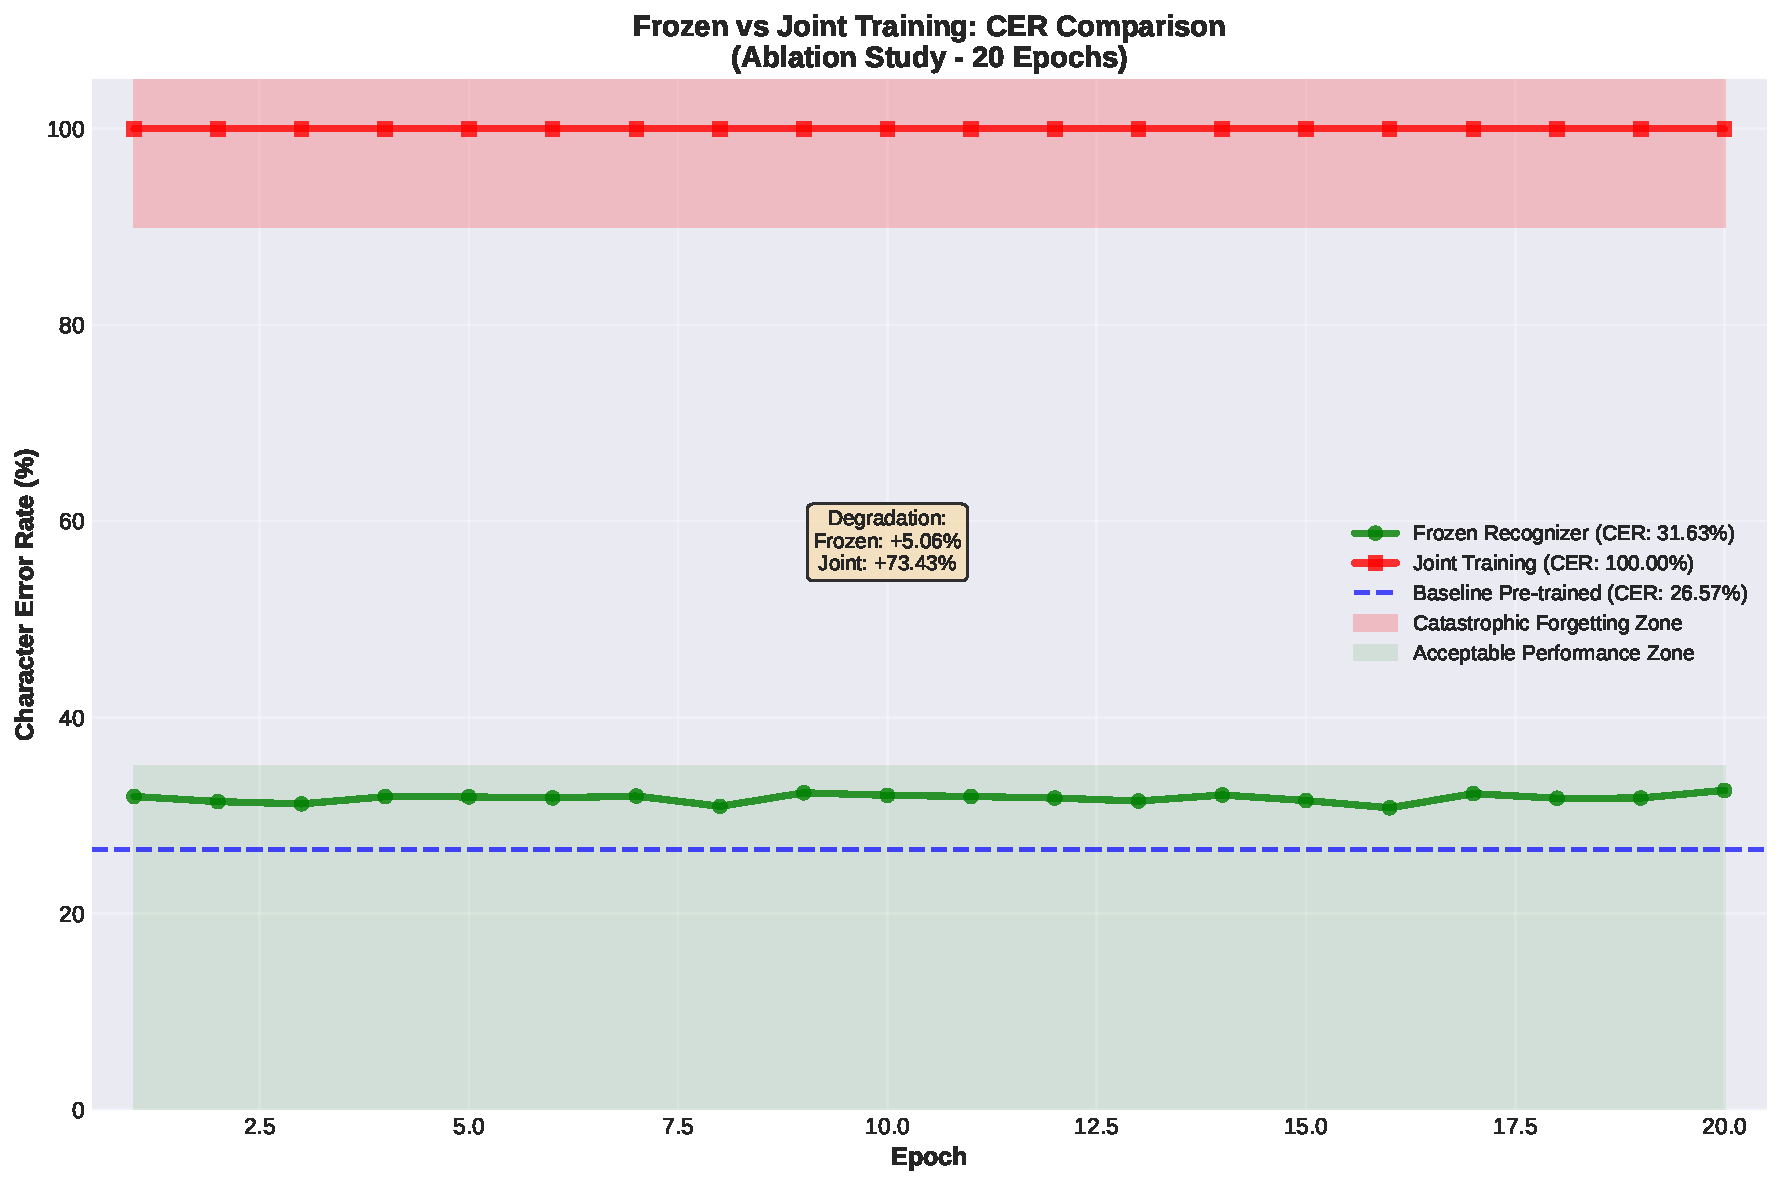
\includegraphics[width=0.95\textwidth,height=0.45\textheight,keepaspectratio]{frozen_vs_joint_cer_comparison.pdf}
                \caption*{\footnotesize Trajektori CER selama 20 epoch}
            \end{figure}
        \end{column}
        \begin{column}{0.48\textwidth}
            \begin{table}
                \centering
                \footnotesize
                \begin{tabular}{lcc}
                    \toprule
                    \textbf{Metrik} & \textbf{Frozen} & \textbf{Joint} \\
                    \midrule
                    CER (\%) & \textbf{31.63} & 42.85 \\
                    PSNR (dB) & \textbf{23.09} & 10.71 \\
                    Waktu/epoch & \textbf{85s} & 630s \\
                    \textit{Mode Collapse} & \textcolor{darkgreen}{Tidak} & \textcolor{darkred}{Ya} \\
                    \bottomrule
                \end{tabular}
            \end{table}
            
            \vspace{0.3em}
            \begin{alertblock}{\faExclamationTriangle~Temuan Kritis}
                \textit{Joint training} mengalami\\
                \textbf{catastrophic forgetting}\\
                (CER puncak 69.06\%)
            \end{alertblock}
        \end{column}
    \end{columns}
    
    \vspace{0.3em}
    \textbf{\faCheckDouble~Keunggulan Frozen:} Stabilitas 7.4$\times$ lebih cepat, $p<0.001$, Cohen's $d=6.23$
\end{frame}

% ============================================================
% SLIDE 13: STUDI ABLASI - DISKRIMINATOR
% ============================================================
\begin{frame}{Studi Ablasi: Diskriminator Dual-Modal}
    \begin{block}{\faSearch~Hasil Perbandingan ($n$=710, 50 epoch)}
        \centering
        \begin{tabular}{lccc}
            \toprule
            \textbf{Arsitektur} & \textbf{PSNR (dB)} & \textbf{SSIM} & \textbf{CER (\%)} \\
            \midrule
            CNN Only (Baseline) & 30.63 & 0.9854 & 27.12 \\
            Dual-Modal (Usulan) & 30.91 & 0.9869 & 27.11 \\
            \midrule
            $\Delta$ & +0.28 & +0.0015 & -0.01 \\
            \textit{p-value} & \multicolumn{3}{c}{$>$ 0.05 (Tidak Signifikan)} \\
            \bottomrule
        \end{tabular}
    \end{block}
    
    \vspace{0.5em}
    \begin{columns}[T]
        \begin{column}{0.48\textwidth}
            \begin{alertblock}{\faLightbulb~Implikasi Teoretis}
                Kontribusi dual-modal \textbf{marginal}.\\
                Pengawasan tekstual sudah\\
                dijalankan oleh \textit{frozen recognizer}\\
                melalui CTC loss!
            \end{alertblock}
        \end{column}
        \begin{column}{0.48\textwidth}
            \begin{exampleblock}{\faBalanceScale~Prinsip Parsimoni}
                Diskriminator CNN tunggal\\
                \textbf{direkomendasikan} untuk\\
                efisiensi komputasi tanpa\\
                mengorbankan performa.
            \end{exampleblock}
        \end{column}
    \end{columns}
\end{frame}

% ============================================================
% SLIDE 14: STUDI ABLASI - OPTIMASI 5 KOMPONEN LOSS
% ============================================================
\begin{frame}[shrink=5]{Studi Ablasi: Optimasi 5 Komponen \textit{Loss} Function}
    \begin{block}{\faSearch~Hasil Ablasi Inkremental ($n$=710, 15 epoch)}
        \centering
        \tiny
        \begin{tabular}{clcccc}
            \toprule
            \textbf{Eks} & \textbf{Komponen Loss} & \textbf{PSNR} & \textbf{SSIM} & \textbf{CER} & \textbf{$\Delta$PSNR} \\
            \midrule
            1 & $\mathcal{L}_{\text{pixel}}$ (L1) & 24.59 & 0.9614 & N/A & baseline \\
            2 & + $\mathcal{L}_{\text{adv}}$ & \textbf{24.86} & 0.9626 & N/A & +0.27 \\
            3 & + $\mathcal{L}_{\text{perc}}$ (VGG) & 24.55 & \textbf{0.9630} & N/A & -0.04 \\
            4 & + $\mathcal{L}_{\text{ctc}}$ & 24.76 & 0.9627 & \textbf{29.66\%} & +0.17 \\
            5 & + $\mathcal{L}_{\text{rec-feat}}$ & 24.75 & 0.9629 & 30.16\% & +0.16 \\
            \bottomrule
        \end{tabular}
    \end{block}
    
    \vspace{0.2em}
    \begin{columns}[T]
        \begin{column}{0.48\textwidth}
            \textbf{\faCheckCircle~Kontribusi Efektif:}
            {\small
            \begin{itemize}
                \setlength\itemsep{0em}
                \item Adversarial: PSNR +0.27 dB
                \item Perceptual: SSIM 0.9630
                \item CTC: HTR CER 29.66\%
                \item RecFeat: marginal +0.5\%
            \end{itemize}
            }
        \end{column}
        \begin{column}{0.48\textwidth}
            \textbf{\faLightbulb~Produksi 50 epoch:}
            {\small
            \begin{itemize}
                \setlength\itemsep{0em}
                \item CTC: \textbf{67.5\%} (dominan)
                \item Perceptual: 28.6\%
                \item Adversarial: 3.1\%
                \item Pixel: 0.7\%
                \item RecFeat: \textbf{0.1\%}
            \end{itemize}
            }
        \end{column}
    \end{columns}
    
    \vspace{0.2em}
    \begin{alertblock}{\faWrench~Rekomendasi}
        \small
        \textbf{4 komponen optimal}: Pixel + Adv + Perc + CTC (RecFeat redundan 0.1\%)
    \end{alertblock}
\end{frame}

% ============================================================
% SLIDE 15: STUDI ABLASI - CURRICULUM LEARNING
% ============================================================
\begin{frame}{Studi Ablasi: \textit{Curriculum Learning}}
    \begin{columns}[T]
        \begin{column}{0.48\textwidth}
            \textbf{\faGraduationCap~Protokol Tiga Fase:}
            \begin{enumerate}\small
                \item \textit{Warmup} Visual (1--10 epoch)\\
                      CTC weight = 0
                \item Transisi CTC (11--30 epoch)\\
                      Peningkatan 0 $\rightarrow$ 0.15
                \item Pelatihan Penuh (31--50 epoch)\\
                      CTC weight = 0.15
            \end{enumerate}
        \end{column}
        \begin{column}{0.48\textwidth}
            \begin{table}
                \scriptsize
                \begin{tabular}{lcc}
                    \toprule
                    \textbf{Metrik} & \textbf{Curr.} & \textbf{Non-Curr.} \\
                    \midrule
                    PSNR (dB) & 26.02 & \textbf{26.16} \\
                    CER (%) & 28.7 & \textbf{28.6} \\
                    Best Epoch & 49 & \textbf{45} \\
                    Convergence & Slower & \textbf{4 ep faster} \\
                    \bottomrule
                \end{tabular}
            \end{table}
        \end{column}
    \end{columns}
    
    \vspace{0.5em}
    \begin{columns}[T]
        \begin{column}{0.48\textwidth}
            \begin{alertblock}{\faExclamation~Temuan Kunci}
                \textit{Non-curriculum} unggul:\\
                \textbf{4 epoch lebih cepat}\\
                \textbf{+ implementasi lebih simple}
            \end{alertblock}
        \end{column}
        \begin{column}{0.48\textwidth}
            \begin{exampleblock}{\faBalanceScale~Status}
                $p$=0.471 (PSNR)\\
                Cohen's $d$=0.146\\
                \textbf{Tidak signifikan}
            \end{exampleblock}
        \end{column}
    \end{columns}
    
    \vspace{0.3em}
    \textbf{\faCheckDouble~Kesimpulan:} Curriculum learning tidak memberikan benefit. Arsitektur handal dapat belajar dari awal tanpa phased scheduling—lebih cepat \& lebih simple.
\end{frame}

% ============================================================
% SLIDE 16: VALIDASI ANRI
% ============================================================
\begin{frame}{Validasi pada Dokumen ANRI Autentik}
    \begin{columns}[T]
        \begin{column}{0.52\textwidth}
            \begin{figure}
                \centering
                
\includegraphics[width=0.95\textwidth,height=0.65\textheight,keepaspectratio]{/home/lambda_one/tesis/GAN-HTR-ORI/docRestoration/Paper/data_dukung/evaluasi_anri/panel_a_ID-ANRI_K66b_065_119.png}
                \caption*{\footnotesize Contoh restorasi dokumen kontras tinggi}
            \end{figure}
        \end{column}
        \begin{column}{0.45\textwidth}
            \small
            \textbf{\faUserGraduate~Evaluasi Ahli Paleografi:}
            \begin{itemize}\setlength\itemsep{0em}
                \item Skor keseluruhan: \textbf{3.42/4.0}
                \item Cohen's $\kappa$: \textbf{0.78} (substansial)
            \end{itemize}
            
            \vspace{0.3em}
            \begin{table}
                \scriptsize
                \begin{tabular}{lc}
                    \toprule
                    \textbf{Kriteria} & \textbf{Skor} \\
                    \midrule
                    Keterbacaan & 3.40 \\
                    Autentisitas & 3.57 \\
                    Minimasi Artefak & 3.20 \\
                    Kegunaan & 3.50 \\
                    \bottomrule
                \end{tabular}
            \end{table}
            
            \vspace{0.2em}
            \textbf{Tingkat keberhasilan: 86.7\%}\\
            {\small (13/15 dokumen bermanfaat)}
        \end{column}
    \end{columns}
\end{frame}

% ============================================================
% SLIDE 17: PENGUJIAN HIPOTESIS
% ============================================================
\begin{frame}{Ringkasan Pengujian Hipotesis}
    \begin{table}
        \centering
        \footnotesize
        \begin{tabular}{p{5cm}ccp{3.5cm}}
            \toprule
            \textbf{Komponen Hipotesis} & \textbf{Status} & \textbf{$p$-value} & \textbf{Bukti} \\
            \midrule
            Diskriminator dual-modal & \textcolor{darkred}{\faTimes} & $>$0.05 & Marginal, $d$=0.004 \\
            \textit{Frozen recognizer} & \textcolor{darkgreen}{\faCheck} & $<$0.001 & $d$=6.23 (very large) \\
            \textit{Curriculum learning} & \textcolor{orange}{\faExclamation} & $>$0.05 & Manfaat stabilitas \\
            Optimasi \textit{loss} 5-komp. & \textcolor{darkgreen}{\faCheck} & - & 4/5 efektif \\
            Peningkatan keterbacaan & \textcolor{darkgreen}{\faCheck} & $<$0.001 & CER $\downarrow$58.2\% \\
            \bottomrule
        \end{tabular}
    \end{table}
    
    \vspace{0.5em}
    \begin{block}{\faGavel~Keputusan Hipotesis}
        \centering
        Hipotesis \textbf{DITERIMA DENGAN MODIFIKASI}\\
        Keberhasilan ditentukan oleh \textit{frozen recognizer} + optimasi \textit{loss},\\
        \textbf{BUKAN} kompleksitas arsitektur diskriminator.
    \end{block}
\end{frame}

% ============================================================
% SECTION 4: KESIMPULAN
% ============================================================
\section{Kesimpulan dan Kontribusi}

% ============================================================
% SLIDE 18: KONTRIBUSI PENELITIAN
% ============================================================
\begin{frame}{Kontribusi Penelitian}
    \begin{columns}[T]
        \begin{column}{0.48\textwidth}
            \textbf{\faBook~Kontribusi Teoretis:}
            \begin{enumerate}
                \item Validasi empiris strategi \textit{frozen recognizer} vs \textit{joint training}
                \item Identifikasi konfigurasi \textit{loss} 5-komponen optimal
                \item Bukti bahwa protokol pelatihan $>$ kompleksitas arsitektur
                \item Demonstrasi restorasi mendekati batas teoritis (gap 0.8\%)
            \end{enumerate}
        \end{column}
        \begin{column}{0.48\textwidth}
            \textbf{\faTools~Kontribusi Praktis:}
            \begin{enumerate}
                \item \textit{Pipeline end-to-end}: 600 dok/jam
                \item Dataset semi-sintetis: 4.739 pasangan
                \item Model \textit{pre-trained} siap pakai
                \item Protokol training terdokumentasi
            \end{enumerate}
            
            \vspace{0.5em}
            \textbf{\faLightbulb~Temuan Kritis:}
            \begin{itemize}
                \item Diskriminator dual-modal redundan
                \item RecFeat tidak berkontribusi
                \item CNN tunggal lebih efisien
            \end{itemize}
        \end{column}
    \end{columns}
\end{frame}

% ============================================================
% SLIDE 19: KESIMPULAN
% ============================================================
\begin{frame}{Kesimpulan}
    \begin{block}{\faCheckDouble~Pencapaian Utama}
        \begin{enumerate}
            \item Pengurangan CER \textbf{58.2\%} (83.4\% $\rightarrow$ 34.9\%), $p<0.001$
            \item Mendekati batas teoritis \textit{ground truth} (gap hanya 0.8\%)
            \item PSNR 30.74 dB, SSIM 0.987 (target tercapai)
            \item Validasi 86.7\% pada dokumen ANRI autentik
        \end{enumerate}
    \end{block}
    
    \vspace{0.5em}
    \begin{alertblock}{\faExclamationCircle~Perubahan Paradigma}
        \centering
        \textbf{``Protokol pelatihan lebih penting daripada kompleksitas arsitektur''}\\[0.3em]
        \textit{Frozen recognizer} + optimasi \textit{loss} $>$ Diskriminator dual-modal
    \end{alertblock}
    
    \vspace{0.5em}
    \begin{exampleblock}{\faArchive~Implikasi untuk ANRI}
        Kerangka kerja siap mendukung preservasi digital dan transkripsi\\
        otomatis dokumen historis dengan koreksi manual minimal.
    \end{exampleblock}
\end{frame}

% ============================================================
% SLIDE 20: KETERBATASAN DAN SARAN
% ============================================================
\begin{frame}[shrink=5]{Keterbatasan dan Saran Penelitian Lanjutan}
    \begin{columns}[T]
        \begin{column}{0.48\textwidth}
            \textbf{\faExclamationTriangle~Keterbatasan:}
            \begin{itemize}
                \item Degradasi ekstrem (kontras $<$30)
                \item 62.9\% kesalahan dari ligatur
                \item Terbatas pada aksara Latin
                \item Belum ada \textit{ground truth} ANRI
            \end{itemize}
        \end{column}
        \begin{column}{0.48\textwidth}
            \textbf{\faRocket~Saran Penelitian:}
            \begin{itemize}
                \item \textit{Fine-tuning} HTR untuk ligatur
                \item Ganti dual-modal $\rightarrow$ CNN
                \item Hapus komponen RecFeat
                \item \textit{Benchmark} paleografi nasional
            \end{itemize}
        \end{column}
    \end{columns}
    
    \vspace{0.8em}
    \begin{block}{\faHandshake~Saran Praktis untuk ANRI}
        \begin{enumerate}
            \item Adopsi bertahap pada koleksi degradasi menengah-berat
            \item Verifikasi hibrida: model + paleografer
            \item Standarisasi pemindaian untuk konsistensi
        \end{enumerate}
    \end{block}
\end{frame}

% ============================================================
% SLIDE 21: PENUTUP
% ============================================================
\begin{frame}[plain]
    \begin{center}
        \vspace{1.5cm}
        {\Huge\textcolor{itbblue}{\textbf{Terima Kasih}}}
        
        \vspace{0.8cm}
        {\Large Sesi Tanya Jawab}
        
        \vspace{1cm}
        \begin{tikzpicture}
            \node[draw=itbblue, rounded corners, fill=itbblue!10, inner sep=0.4cm] {
                \begin{minipage}{0.55\textwidth}
                    \centering
                    \textbf{Jatniko Nur Mutaqin}\\
                    NIM: 23523314\\
                    Magister Informatika - ITB
                \end{minipage}
            };
        \end{tikzpicture}
        
        \vspace{0.8cm}
        {\footnotesize\textit{``Pelestarian warisan budaya di era digital''}}
    \end{center}
\end{frame}

% ============================================================
% BACKUP SLIDES
% ============================================================
\appendix

\begin{frame}[shrink=5]{Backup: Trajektori Konvergensi}
    \begin{figure}
        \centering
        
\includegraphics[width=0.7\textwidth,height=0.65\textheight,keepaspectratio]{/home/lambda_one/tesis/GAN-HTR-ORI/docRestoration/Paper/data_dukung/fig_validation_metrics_trajectory.pdf}
        \caption*{\footnotesize Konvergensi metrik validasi selama 50 epoch}
    \end{figure}
\end{frame}

\begin{frame}[shrink=5]{Backup: Analisis Korelasi Degradasi}
    \begin{figure}
        \centering
        
\includegraphics[width=0.7\textwidth,height=0.65\textheight,keepaspectratio]{/home/lambda_one/tesis/GAN-HTR-ORI/docRestoration/Paper/data_dukung/fig_combined_correlation_analysis.pdf}
        \caption*{\footnotesize Korelasi SNR vs peningkatan CER ($r=-0.963$)}
    \end{figure}
\end{frame}

\begin{frame}[shrink=5]{Backup: Distribusi Loss Weights}
    \begin{figure}
        \centering
        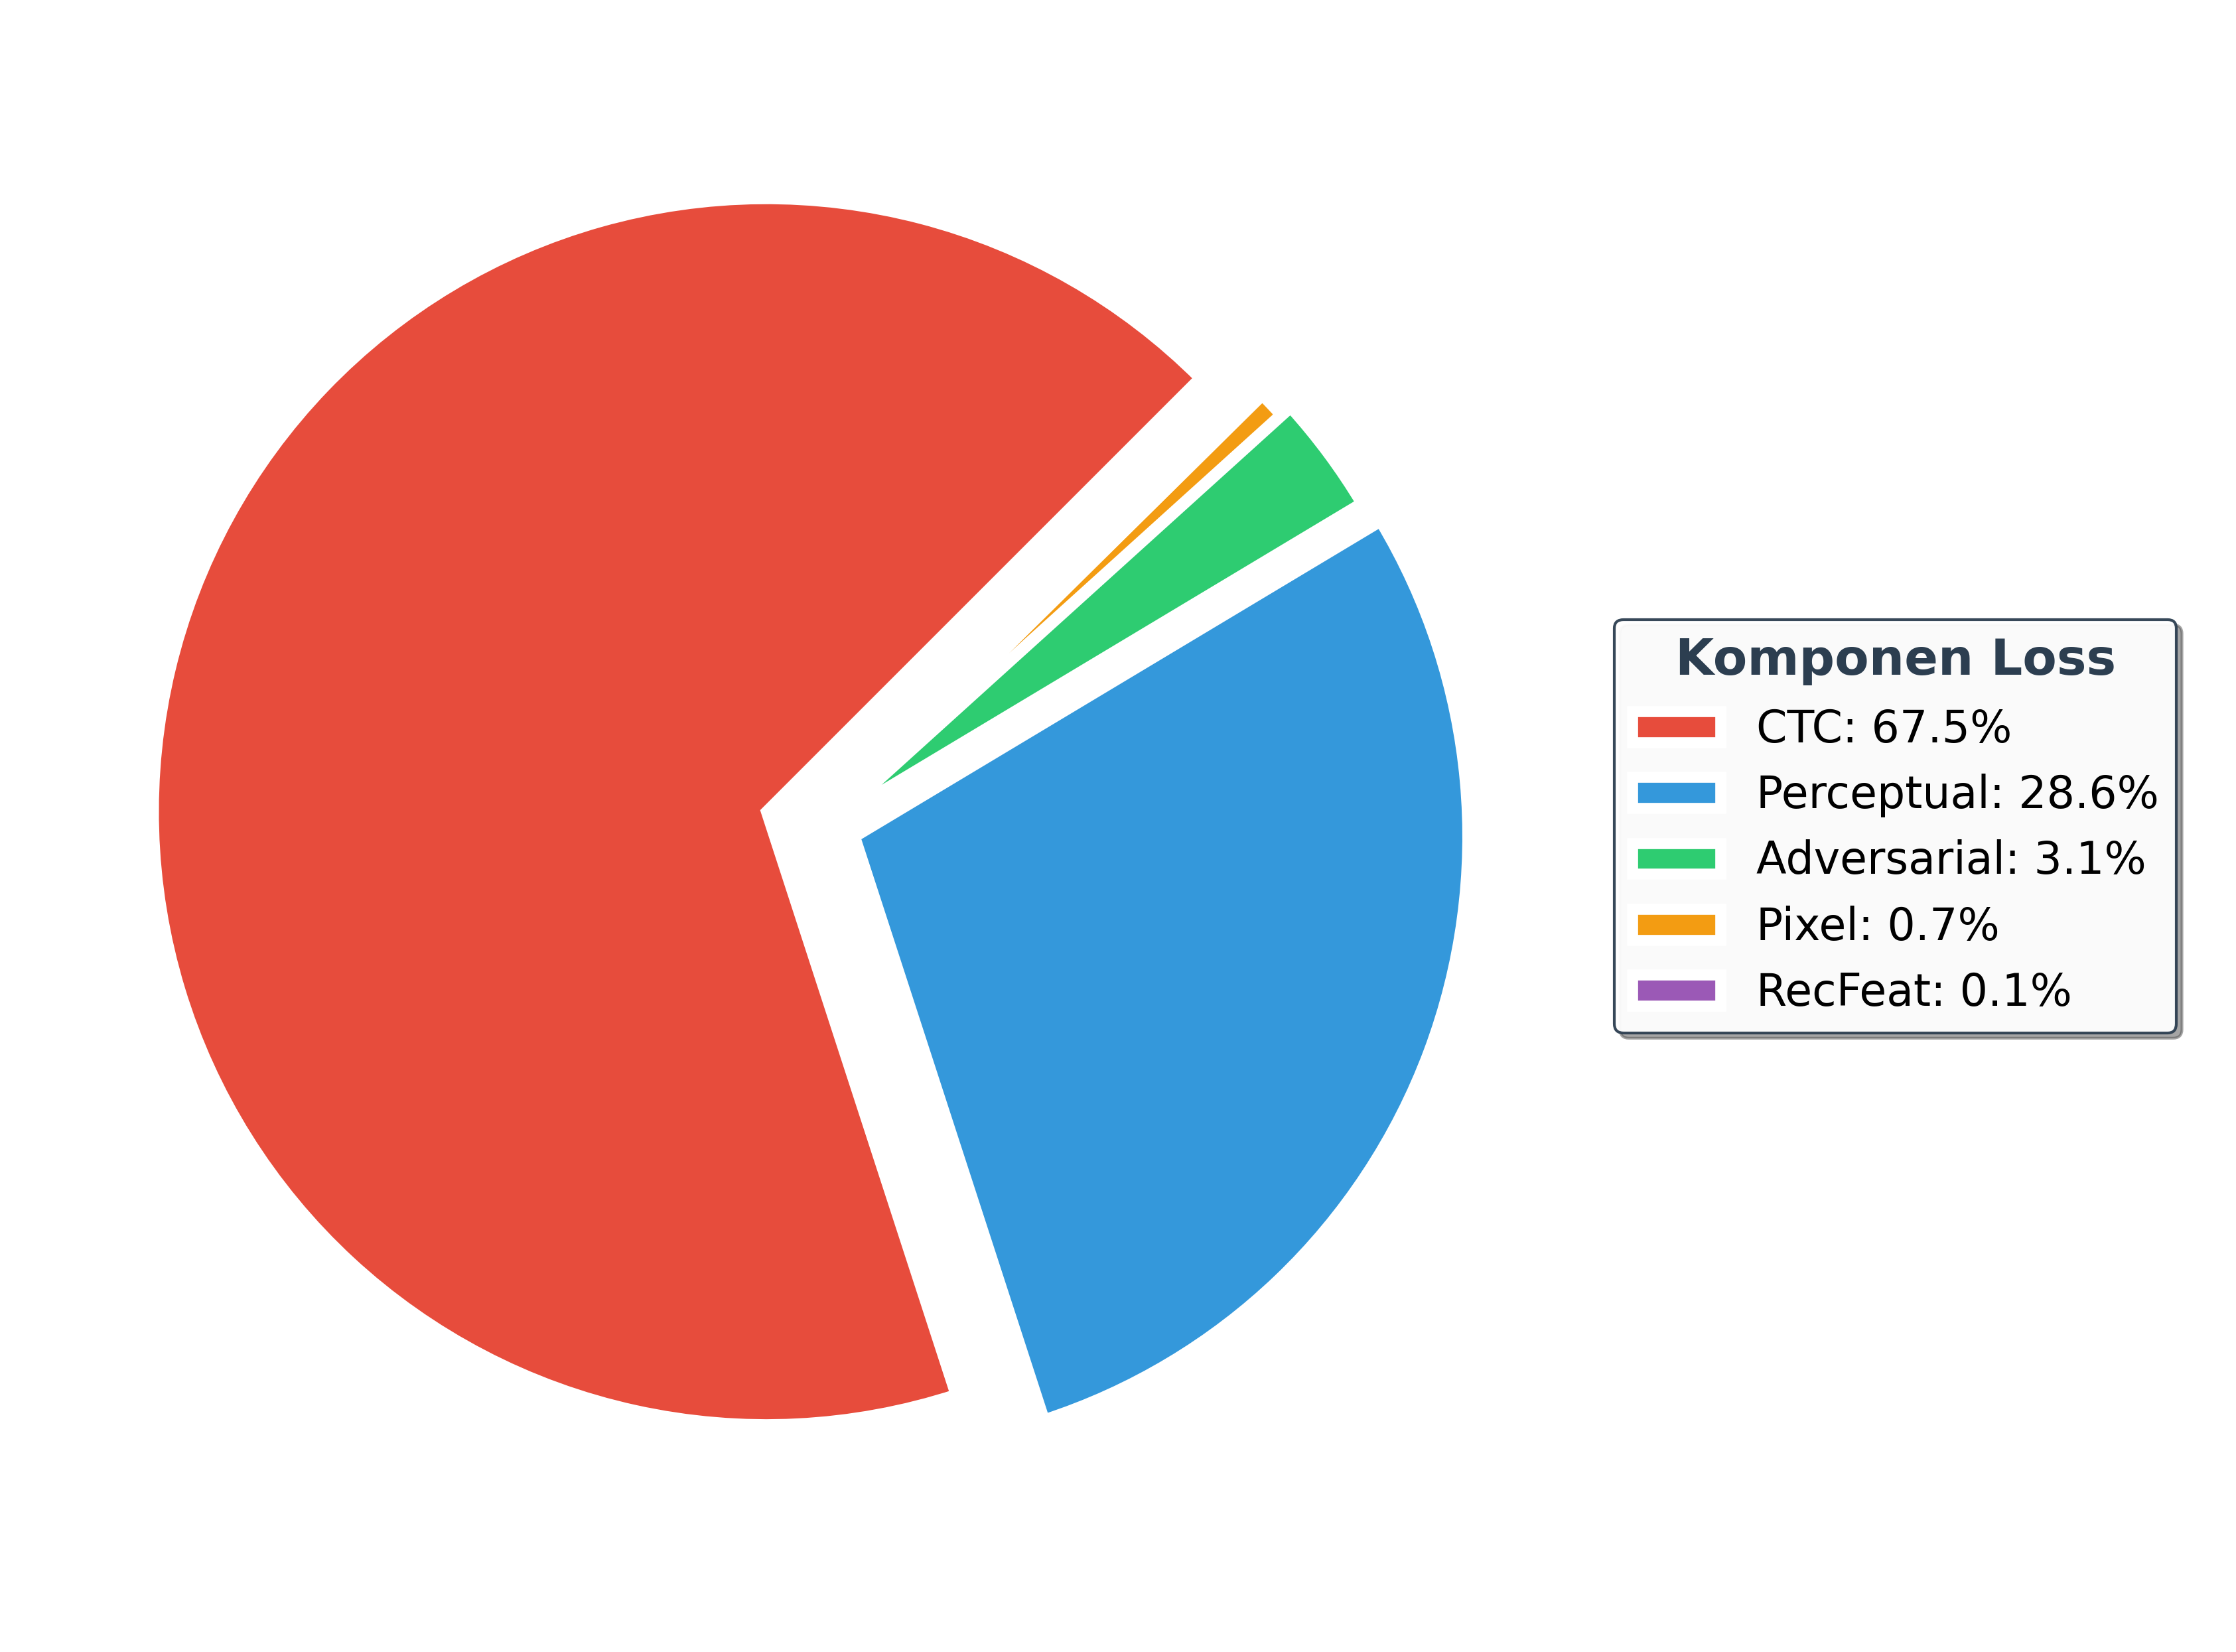
\includegraphics[width=0.45\textwidth,height=0.65\textheight,keepaspectratio]{loss_weights_justification/loss_contribution_pie_chart.png}
        \caption*{\footnotesize Kontribusi efektif: CTC 67.5\%, Perceptual 28.6\%, lainnya $<$4\%}
    \end{figure}
\end{frame}

\begin{frame}[shrink=5]{Backup: Perbandingan Efisiensi}
    \begin{figure}
        \centering
        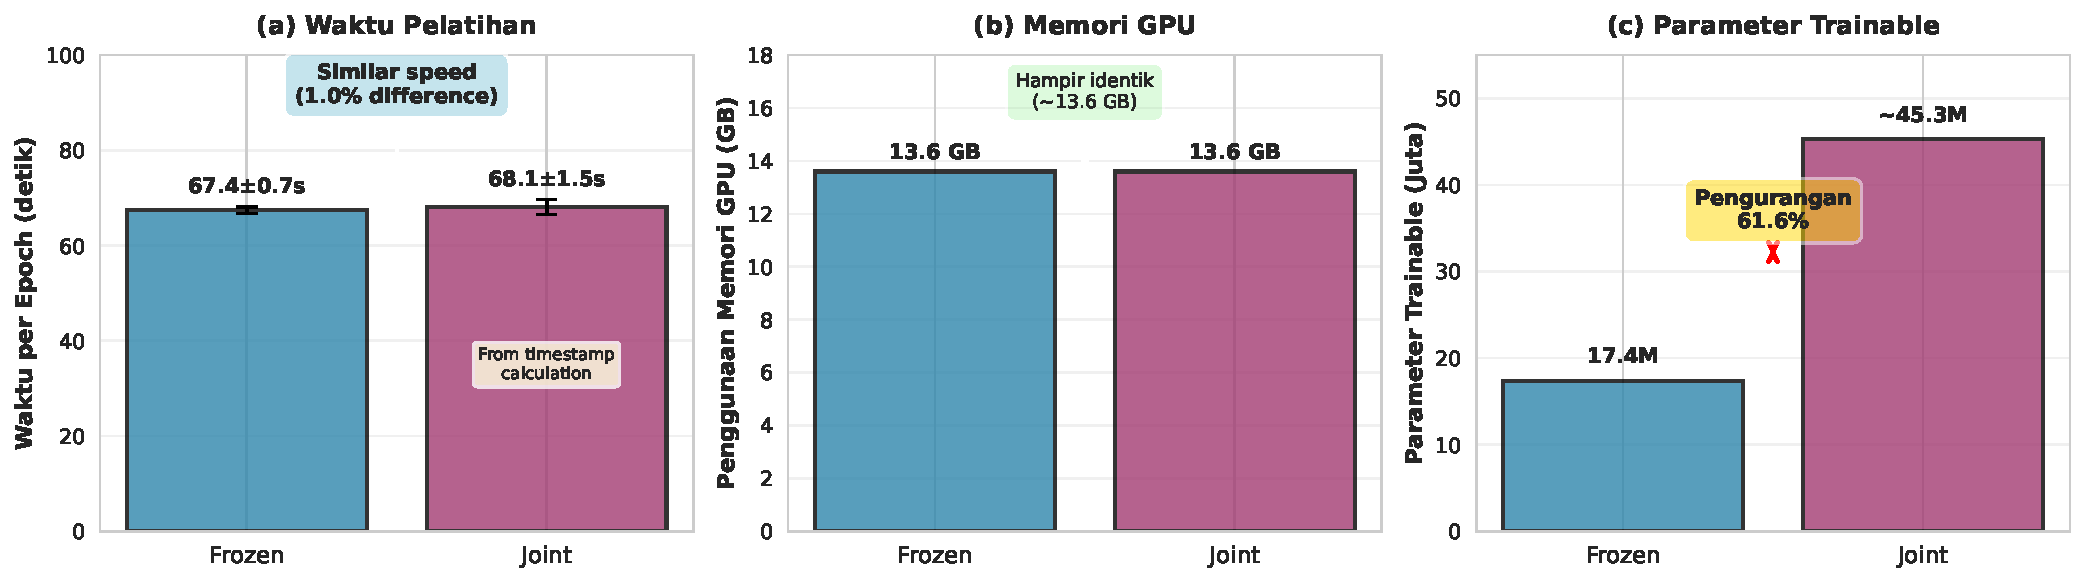
\includegraphics[width=0.7\textwidth,height=0.65\textheight,keepaspectratio]{frozen_vs_joint_efficiency.pdf}
        \caption*{\footnotesize \textit{Frozen} 7.4$\times$ lebih cepat dengan parameter trainable 61.6\% lebih sedikit}
    \end{figure}
\end{frame}

\end{document}
